\begin{enumerate}[\Large\bfseries 1.]

%--------------------1.
\item \textbf{\large APLICACIÓN DE INTEGRALES}\\\\

    \begin{enumerate}[\bfseries a)]

	%----------a.
	\item \textbf{\large Tom Apostol, Calculus I, Capítulo 2, Problema 32}\\\\
	A partir de la identidad 
	    $$2\sen \dfrac{x}{2} \cos kx = \sen(2k+1)\dfrac{x}{2} - \sen(2k-1)\dfrac{x}{2}$$
	    y de las propiedades telescópicas de las sumas finitas demostrar que si $x\neq 2m$ (m entero) se tiene
	    $$\sum_{k=1}^n \cos kx = \dfrac{\sen \frac{1}{2}nx\cos \frac{1}{2}(n+1)x}{\sen\frac{1}{2}x}$$\\
	    Demostración.-\; Haciendo $k= 1,2,\ldots, n$ y sumando esas igualdades, se obtiene que
	    $$2\sen \dfrac{x}{2} \sum_{k=1}^n \cos kx = \sum_{k=1}^n \left[\sen(2k+1)\dfrac{x}{2} - \sen(2k-1)\dfrac{x}{2}\right]$$
	    Luego por la propiedad telescopica de las sumas finitas, se tiene, 
	    $$2\sen\dfrac{\pi}{2}\sum\limits_{k=1}^n \cos kx = \sen \left[(2n+1)\dfrac{x}{2}\right]-\sen(0+1)\dfrac{x}{2}$$
	    luego,
	    $$\begin{array}{rcl}
		\displaystyle\sum_{k=1}^n \cos kx&=&\dfrac{\sen \left[(2n+1)\frac{x}{2}\right]-\sen\frac{x}{2}}{2\sen \frac{x}{2}}\\\\
						 &=&\dfrac{2\sen\frac{(2n+1)\frac{x}{2}-\frac{x}{2}}{2}\cos \frac{(2n+1)\frac{x}{2}+\frac{x}{2}}{2}}{2\sen\frac{x}{2}}\\\\
						 &=&\dfrac{\sen\frac{nx}{2}\cos\frac{(n+1)x}{2}}{\sen\frac{x}{2}}\\\\
	    \end{array}$$

	%----------b)
	\item \textbf{Código fuente.}\\ 
	    
	    \lstinputlisting[language=Python]{python/tareas_mat/week7/py32.py}
	    \vspace{.5cm}
	
	%----------c)
	\item \textbf{Prueba de la ejecución del programa}.\\
	    \begin{center}
		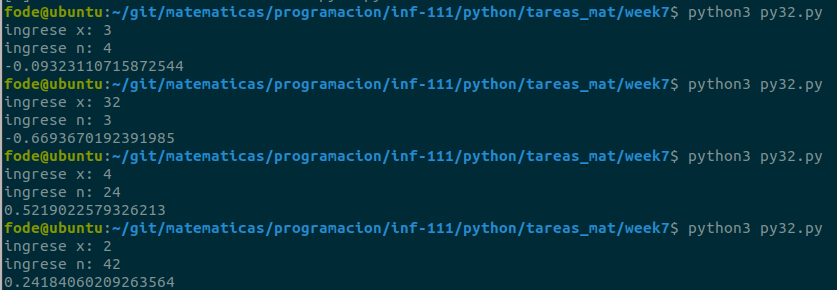
\includegraphics[scale=.55]{imagenes/tareas_mat/week7/py32.png}
	    \end{center}

    \end{enumerate}

\newpage

%--------------------2.
\item \textbf{\large APLICACIÓN DE INTEGRALES}\\\\

    \begin{enumerate}[\bfseries a)]

	%----------a.
	\item \textbf{\large Tom Apostol, Calculus I, Capítulo 2, Problema 20}\\\\
	    $\displaystyle\int_0^{\pi/2} (\sen x - \cos x)\; dx = 1-\cos \left(\dfrac{\pi}{2}\right) - \sen\left(\dfrac{\pi}{2}\right) = 1-0-1 = 0$.\\\\

	%----------b)
	\item \textbf{Código fuente.}\\ 
	    
	    \lstinputlisting[language=Python]{python/tareas_mat/week7/py20.py}
	    \vspace{.5cm}
	
	%----------c)
	\item \textbf{Prueba de la ejecución del programa}.\\
	    \begin{center}
		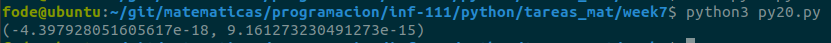
\includegraphics[scale=.55]{imagenes/tareas_mat/week7/py20.png}
	    \end{center}

    \end{enumerate}

\newpage

%--------------------3.
\item \textbf{\large APLICACIÓN DE INTEGRALES}\\\\

    \begin{enumerate}[\bfseries a)]

	%----------a.
	\item \textbf{\large Tom Apostol, Calculus I, Capítulo 2, Problema 33}\\\\
	Si $x\neq 2m\pi$ ($m$ un entero), probar que 
	    $$\sum\limits_{k=1}^n \sen kx = \dfrac{\sen\frac{1}{2} nx \sen\frac{1}{2}(n+1)x}{\sen\frac{1}{2}x}$$\\
	    Demostración.-\; Recordemos que 
	    $$\begin{array}{rcl}
	    -2\sen\dfrac{x}{2}\sen(kx)&=&\cos\left(\dfrac{x}{2}+kx\right) - \cos\left(\dfrac{x}{2}-kx\right)\\\\
				      &=&\cos\left[(2k+1)\dfrac{x}{2}\right]-\cos\left[(1-2k)\dfrac{x}{2}\right]\\\\
				      &=&\cos \left[(2k+1)\dfrac{x}{2}\right]-\cos\left[(2k-1)\dfrac{x}{2}\right]\\\\
	    \end{array}$$
	    
	    Luego, aplicando la propiedad telescópica de las sumas finitas, y la primera parte del teorema 4 se tiene,
	    $$\begin{array}{rcl}
		\sum\limits_{k=1}^n \sen kx&=&\dfrac{\cos \left[(n+\frac{1}{2})\right]-\cos \frac{x}{2}}{-2\sen \frac{x}{2}}\\\\
					   &=&\dfrac{\cos(nx)\cos \frac{x}{2}-\sen(mx)\sen \frac{x}{2}-\cos \frac{x}{2}}{-2\sen \frac{x}{2}}\\\\
					   &=&\dfrac{\cos\frac{x}{2}(\cos(nx)-1)-\sen (nx) \sen \frac{x}{2}}{-2\sen \frac{x}{2}}\\\\
					   &=&\dfrac{-2\cos \frac{x}{2}\sen^2 \frac{nx}{2} - 2\sen \frac{ns}{2} \cos \frac{nx}{2} \sen \frac{x}{2}}{-2\sen \frac{x}{2}}\\\\
					   &=&\dfrac{\sen \frac{nx}{2}\left(\cos \frac{x}{2} \sen \frac{nx}{2} + \cos \frac{nx}{2} \sen{x}{2}\right)}{2\sen \frac{x}{2}}\\\\
					   &=&\dfrac{\sen \frac{nx}{2} \sen \frac{(n+1)x}{2}}{2\sen \frac{x}{2}}\\\\
	    \end{array}$$

	%----------b)
	\item \textbf{Código fuente.}\\ 
	    
	    \lstinputlisting[language=Python]{python/tareas_mat/week7/py33.py}
	    \vspace{.5cm}
	
	%----------c)
	\item \textbf{Prueba de la ejecución del programa}.\\
	    \begin{center}
		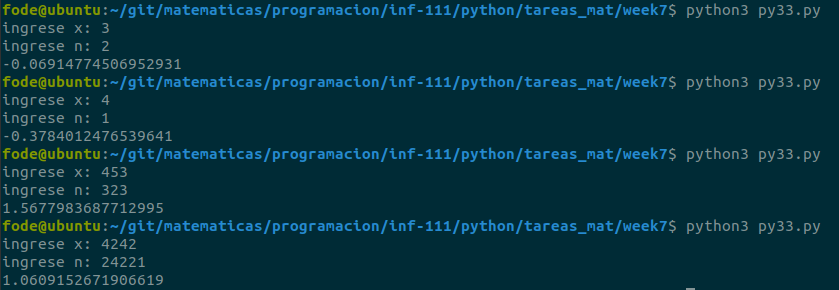
\includegraphics[scale=.55]{imagenes/tareas_mat/week7/py33.png}
	    \end{center}

    \end{enumerate}

\newpage

%--------------------4.
\item \textbf{\large APLICACIÓN DE INTEGRALES}\\\\

    \begin{enumerate}[\bfseries a)]

	%----------a.
	\item \textbf{\large Tom Apostol, Calculus I, Capítulo 2, Problema 18}\\\\
	$\displaystyle\int_{0}^\pi (x+\sen x)\; dx = \dfrac{x^2}{2}\bigg|_0^\pi + 1 - (\cos \pi) = \dfrac{\pi^2}{2}+1-(-1) = \dfrac{\pi^2}{2} + 2$.\\\\
	%----------b)
	\item \textbf{Código fuente.}\\ 
	    
	    \lstinputlisting[language=Python]{python/tareas_mat/week7/py18.py}
	    \vspace{.5cm}
	
	%----------c)
	\item \textbf{Prueba de la ejecución del programa}.\\
	    \begin{center}
		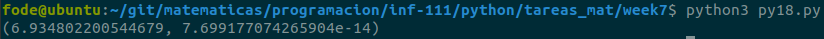
\includegraphics[scale=.55]{imagenes/tareas_mat/week7/py18.png}
	    \end{center}

    \end{enumerate}

\newpage

%--------------------5.
\item \textbf{\large APLICACIÓN DE INTEGRALES}\\\\

    \begin{enumerate}[\bfseries a)]

	%----------a.
	\item \textbf{\large Tom Apostol, Calculus I, Capítulo 2, Problema 19}\\\\
	$\displaystyle\int_{0}^{\pi/2} (x^2+\cos x)\; dx = \dfrac{x^3}{3}\bigg|_0^{\pi/2}+\sen\left(\dfrac{\pi}{2}\right) = \dfrac{(\frac{\pi}{2})^3}{3} + 1 = \dfrac{\pi^3}{24}+1.$\\\\

	%----------b)
	\item \textbf{Código fuente.}\\ 
	    
	    \lstinputlisting[language=Python]{python/tareas_mat/week7/py19.py}
	    \vspace{.5cm}
	
	%----------c)
	\item \textbf{Prueba de la ejecución del programa}.\\
	    \begin{center}
		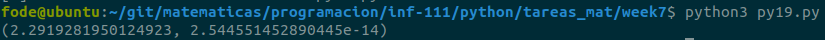
\includegraphics[scale=.55]{imagenes/tareas_mat/week7/py19.png}
	    \end{center}

    \end{enumerate}

\newpage
\end{enumerate}
